%!TEX root = ../Thesis.tex

\section{Problem 1}
\label{sec:problem_1}%

The scope of this problem is to illustrate the MATLAB implementation of the BEM by solving a simple potential problem for the Laplace equation in the unit square domain $\Omega$ under mixed boundary conditions as shown in Figure~\ref{fig:2pr1f1}.

\begin{figure}[H]
    \centering
    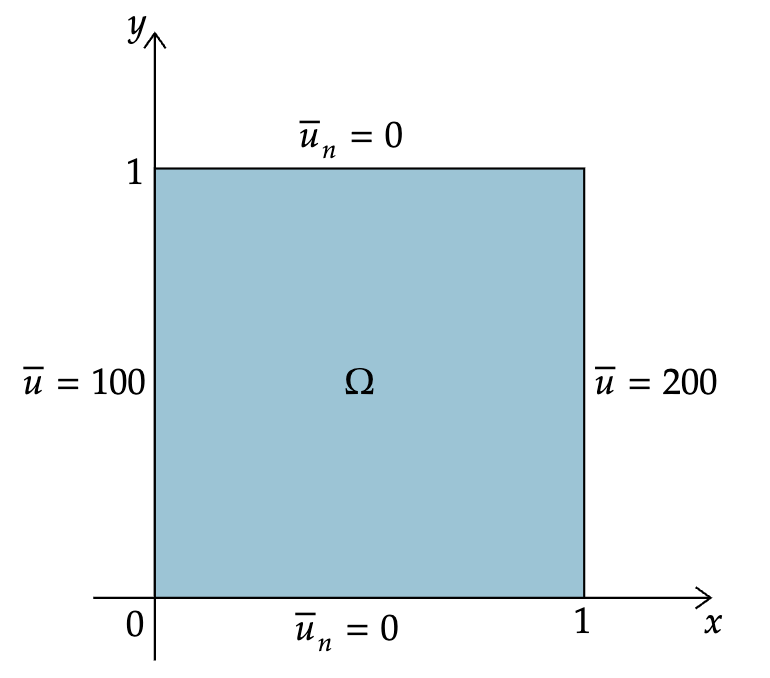
\includegraphics[width=0.5\textwidth]{pr1f1}
    \caption{Square domain $\Omega$ and boundary conditions of Problem 1.}
    \label{fig:2pr1f1}
\end{figure}


\subsection{MATLAB Implementation}
\label{sub:MATLAB_implementation2}%

We start with a very coarse grid, namely made with a number of elements $\text{N}=16$. In Table~\ref{table:2pr1t1} we explain the other inputs:
\begin{table}[H]
    %\caption*{\textbf{Title of Table (optional)}}
    \centering 
    \begin{tabular}{cl}
    \hline
    \rowcolor{bluepoli!40} % comment this line to remove the color
    Variable & Meaning  \\
    \hline
    N & Number of boundary elements and boundary nodes \\
    IN & Number of internal points where the solution is computed \\
    XL & One-dimensional array containing the $x$ coordinates \\
    & of the extreme points of all the elements \\
    YL & One-dimensional array containing the $y$ coordinates \\
    & of the extreme points of all the elements \\
    XIN & One-dimensional array containing the $x$ coordinates \\
    & of the internal points at which te values of $u$ are computed \\
    YIN & One-dimensional array containing the $y$ coordinates \\
    & of the internal points at which te values of $u$ are computed \\
    INDEX & One-dimensional boolean array in which a type of \\
    & boundary condition is assigned to the nodes \\
    UB & One-dimensional array containing the boundary values \\
    & of $u$, if INDEX=0, or $\partial u / \partial n$, if INDEX=1 \\
    \hline
    \end{tabular}
    \\[10pt]
    \caption{Inputs for the MATLAB program.}
    \label{table:2pr1t1}
\end{table}

We immediately compute the $x$ and $y$ coordinates of all the boundary nodes thanks to the \texttt{MIDPOINTS} function (Algorithm~\ref{alg:MIDPOINTS}), and we store them into XM and YM arrays.

Hence, the initial discretization, as the \texttt{INPUT} function (Algorithm that just prints the input data) can confirm, looks like this:
\begin{figure}[H]
    \centering
    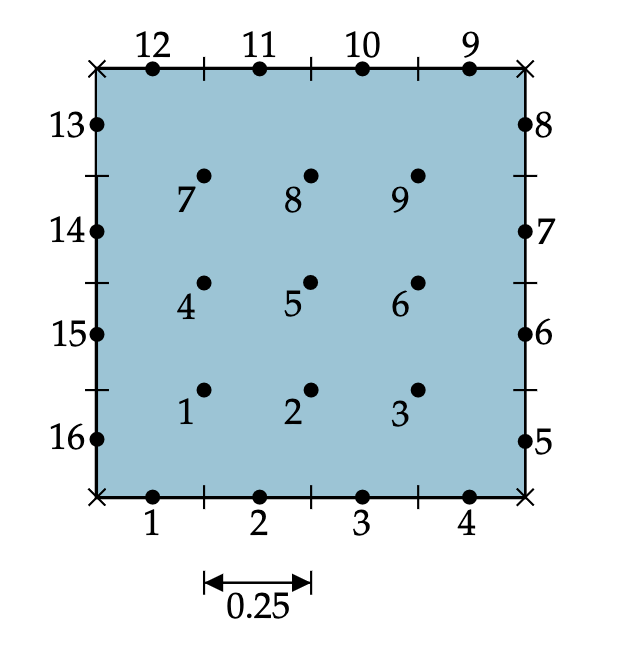
\includegraphics[width=0.4\textwidth]{pr1f2}
    \caption{Boundary element discretization and internal points of Problem 1.}
    \label{fig:2pr1f1}
\end{figure}

Then we compute the $G$ matrix with Algorithm~\ref{alg:GMATR} and the $H$ matrix with Algorithm~\ref{alg:HMATR}. The line intelgrals are computed locally by using the auxiliary Algorithms~\ref{alg:RLINTC},~\ref{alg:SLINTC},~\ref{alg:DALPHA}.

The function \texttt{ABMATR} (Algorithm~\ref{alg:ABMATR}) generates the matrix $A$ and the vector $b$ of Eq.~\eqref{eq:finalAx=b}. Thus, we solve the system with the \emph{backslash} command. 

With Algorithm~\ref{alg:REORDER} we rearrange the solutions according to the INDEX vector, and we finally obtain the solutions vector UB and UNB containing the values of $u$ and $\partial u / \partial n$ on the boundary points.

Finally, we compute the internal values of $u$ thanks to Algorithm~\ref{alg:UINTER} and we print the results with the \texttt{OUTPUT} function.

To sum up, the pseudocode of our program is the following:
\begin{equation}
\label{eq:flowchart}
\begin{gathered}
\text{ INPUT } \to \text{ MIDPOINTS } \to \text{ GMATR } \to \text{ HMATR } \to \text{ ABMATR } \\
 \to \textit{ solve the system (backslash) } \to \text{ REORDER } \to \text{ UINTER } \to \text{ OUTPUT }  
\end{gathered}
\end{equation}

\newpage

The script we run is \texttt{main21} (Algorithm~\ref{alg:main21}), and we obtain the following output:
\begin{matlaboutput}
*********************************************************************
RESULTS
*********************************************************************

BOUNDARY NODES:

NODE        XM            YM            U             U_n
 1        0.12500       0.00000     111.87694       0.00000
 2        0.37500       0.00000     137.32269       0.00000
 3        0.62500       0.00000     162.67731       0.00000
 4        0.87500       0.00000     188.12306       0.00000
 5        1.00000       0.12500     200.00000     105.52311
 6        1.00000       0.37500     200.00000      98.41687
 7        1.00000       0.62500     200.00000      98.41687
 8        1.00000       0.87500     200.00000     105.52311
 9        0.87500       1.00000     188.12306       0.00000
 10       0.62500       1.00000     162.67731       0.00000
 11       0.37500       1.00000     137.32269       0.00000
 12       0.12500       1.00000     111.87694       0.00000
 13       0.00000       0.87500     100.00000    -105.52311
 14       0.00000       0.62500     100.00000     -98.41687
 15       0.00000       0.37500     100.00000     -98.41687
 16       0.00000       0.12500     100.00000    -105.52311

INTERNAL POINTS:

POINT        XIN           YIN           U
  1        0.25000       0.25000     124.88609
  2        0.50000       0.25000     150.00000
  3        0.75000       0.25000     175.11391
  4        0.25000       0.50000     124.95125
  5        0.50000       0.50000     150.00000
  6        0.75000       0.50000     175.04875
  7        0.25000       0.75000     124.88609
  8        0.50000       0.75000     150.00000
  9        0.75000       0.75000     175.11391
\end{matlaboutput}

These results perfectly match the ones obtained with FORTRAN in~\cite{sbemKatsi}. Both of them can be compared with the exact solution $u(x,y)=100(1+x)$, showing a rapid convergence.

\newpage 

\subsection{MATLAB scripts}
\label{sub:matlab_scripts2}%

\begin{matlab}{MIDPOINTS}{alg:MIDPOINTS}
function [XM, YM] = MIDPOINTS(XL, YL, N)
xl = [XL; XL(1)];
yl = [YL; YL(1)];
XM = zeros(N,1);
YM = zeros(N,1);
for i = 1:N
    XM(i) = (xl(i)+xl(i+1))/2;
    YM(i) = (yl(i)+yl(i+1))/2;
end
end
\end{matlab}

\begin{matlab}{GMATR}{alg:GMATR}
function G = GMATR(XL, YL, XM, YM, N)
G = zeros(N,N);
for i = 1:N
    for j = 1:N
        if i ~= j % off-diagonal elements of G
            if j==N
                G(i,j) = RLINTC(XM(i),YM(i),XL(j),YL(j),XL(1),YL(1));
            else
                G(i,j) = RLINTC(XM(i),YM(i),XL(j),YL(j),XL(j+1),YL(j+1));
            end
        elseif i == j % diagonal elements of G
            if j==N
                G(i,j) = SLINTC(XL(j),YL(j),XL(1),YL(1));
            else
                G(i,j) = SLINTC(XL(j),YL(j),XL(j+1),YL(j+1));
            end
        end
    end
end
end
\end{matlab}

\begin{matlab}{HMATR}{alg:HMATR}
function H = HMATR(XL, YL, XM, YM, N)
H = zeros(N,N);
for i = 1:N
    for j = 1:N
        if i ~= j % off-diagonal elements of H
            if j==N
                H(i,j) = DALPHA(XM(i),YM(i),XL(j),YL(j),XL(1),YL(1));


            else
                H(i,j) = DALPHA(XM(i),YM(i),XL(j),YL(j),XL(j+1),YL(j+1));
            end
        elseif i == j % diagonal elements of H
            H(i,j) = -0.5;
        end
    end
end
end
\end{matlab}

\begin{matlab}{RLINTC}{alg:RLINTC}
function result = RLINTC(x0, y0, x1, y1, x2, y2)
% Define Gauss integration points and weights
xi = [-0.86113631,-0.33998104,0.33998104,0.86113631];
wg = [0.34785485,0.65214515,0.65214515,0.34785485];
xc = zeros(4,1);
yc = zeros(4,1);
% Compute constants
ax = (x2-x1)/2;
ay = (y2-y1)/2;
bx = (x2+x1)/2;
by = (y2+y1)/2;
% Compute the line integral
result = 0;
for i = 1:4
    xc(i) = ax*xi(i) + bx;
    yc(i) = ay*xi(i) + by;
    ra = sqrt((xc(i)-x0)^2 + (yc(i)-y0)^2);
    result = result + log(ra)*wg(i);
end
sl = 2*sqrt(ax^2 + ay^2);
result = result*sl/(4*pi);
end
\end{matlab}

\begin{matlab}{SLINTC}{alg:SLINTC}
function result = SLINTC(x1, y1, x2, y2)
% Compute constants
ax = (x2-x1)/2;
ay = (y2-y1)/2;
sl = sqrt(ax^2 + ay^2);
% Compute the line integral
result = sl*(log(sl)-1)/pi;
end
\end{matlab}

\begin{matlab}{DALPHA}{alg:DALPHA}
function result = DALPHA(x0, y0, x1, y1, x2, y2)
% Compute constants
dy1 = y1 - y0;
dx1 = x1 - x0;
dy2 = y2 - y0;
dx2 = x2 - x0;
dl1 = sqrt(dx1^2 + dy1^2);
cos1 = dx1/dl1;
sin1 = dy1/dl1;
dx2r = dx2*cos1 + dy2*sin1;
dy2r = -dx2*sin1 + dy2*cos1;
da = atan2(dy2r,dx2r);
% Compute the line integral
result = da/(2*pi);
end
\end{matlab}

\begin{matlab}{ABMATR}{alg:ABMATR}
function [A, UNB] = ABMATR(G, H, UB, INDEX)
n = size(G,1);
A = zeros(n,n);
UNB = zeros(n,1);
% Reorder the columns of the system of equations and store them in A
for j = 1:n
    if INDEX(j) == 0
        A(:,j) = -G(:,j);
    else
        A(:,j) = H(:,j);
    end
end
% Compute the right-hand side vector and store it in UNB
for i = 1:n
    for j = 1:n
        if INDEX(j) == 0
            UNB(i) = UNB(i) - H(i,j)*UB(j);
        else
            UNB(i) = UNB(i) + G(i,j)*UB(j);
        end
    end
end
end
\end{matlab}

\begin{matlab}{REORDER}{alg:REORDER}
function [UB, UNB] = REORDER(UB, UNB, INDEX)


n = length(UB);
% Rearrange the arrays
for i = 1:n
    if INDEX(i) ~= 0
        ch = UB(i);
        UB(i) = UNB(i);
        UNB(i) = ch;
    end
end
end
\end{matlab}

\begin{matlab}{UINTER}{alg:UINTER}
function UIN = UINTER(XL, YL, XIN, YIN, UB, UNB, N, IN)
UIN = zeros(IN, 1);
for k = 1:IN
    for j = 1:N
        if j==N
            resh = DALPHA(XIN(k), YIN(k), XL(j), YL(j), XL(1), YL(1));
            resg = RLINTC(XIN(k), YIN(k), XL(j), YL(j), XL(1), YL(1));
        else
            resh = DALPHA(XIN(k), YIN(k), XL(j), YL(j), XL(j+1), YL(j+1));
            resg = RLINTC(XIN(k), YIN(k), XL(j), YL(j), XL(j+1), YL(j+1));
        end
        UIN(k) = UIN(k) + resh*UB(j) - resg*UNB(j);
    end
end
end
\end{matlab}

\begin{matlab}{main21}{alg:main21}
%% Problem 1 - Benchmark
clear; clc; 

% Set the maximum dimensions
N = 16;
IN = 9;

% Set data
XL = [0; 0.25; 0.5; 0.75; 1; 1; 1; 1; 1; 0.75; 0.5; 0.25; 0; 0; 0; 0];
YL = [0; 0; 0; 0; 0; 0.25; 0.5; 0.75; 1; 1; 1; 1; 1; 0.75; 0.5; 0.25];
XIN = [0.25; 0.5; 0.75; 0.25; 0.5; 0.75; 0.25; 0.5; 0.75];
YIN = [0.25; 0.25; 0.25; 0.5; 0.5; 0.5; 0.75; 0.75; 0.75];
INDEX = [1; 1; 1; 1; 0; 0; 0; 0; 1; 1; 1; 1; 0; 0; 0; 0];


UB = [0; 0; 0; 0; 200; 200; 200; 200; 0; 0; 0; 0; 100; 100; 100; 100];

% Compute midpoints
[XM, YM] = MIDPOINTS(XL, YL, N);

% Print data
INPUT(XL, YL, XM, YM, XIN, YIN, INDEX, UB, N, IN);

% Compute the G matrix
G = GMATR(XL, YL, XM, YM, N);

% Compute the H matrix
H = HMATR(XL, YL, XM, YM, N);

% Form the system of equations AX=B
[A, UNB] = ABMATR(G, H, UB, INDEX);

% Solve the system of equations
UNB = A\UNB;

% Form the vectors U and UN of all the boundary values
[UB, UNB] = REORDER(UB, UNB, INDEX);

% Compute the values UIN of u at the internal points
UIN = UINTER(XL, YL, XIN, YIN, UB, UNB, N, IN);

% Print results
OUTPUT(XM, YM, XIN, YIN, UB, UNB, UIN, N, IN);

\end{matlab}

\newpage

